\subsection{Architecture}

Our architecture must be multilayered so that small, limited devices may be supported by more powerful hubs. Most of our potential use cases require that information be aggregated at some central cloud-based server. Therefore, we have chosen to implement a three layer hierarchical network of devices [see figure \ref{fig:simplified_architecture}]. At the bottom of the hierarchy are Edge Devices; microcontrollers with low memory, power and connectivity which are not capable of storing and/or transmitting large cryptographic keys or executing secure cryptographic algorithms. Moving up the pyramid, a group of local edge devices may be managed by a single Smart Agent, a more powerful device with an operating system and full TCP/IP network connectivity. At the top of the hierarchy are Cloud Agents; devices and applications that operate in the cloud. These devices link Smart Agents together, provide telemetry, monitoring and data aggregation and can take coordinated action in the event of a suspected attack on the network.

\paragraph{}
This architecture represents a very simplified version of the full mF2C architecture that is being developed by our partners.


\begin{figure}[h]
  \centering
    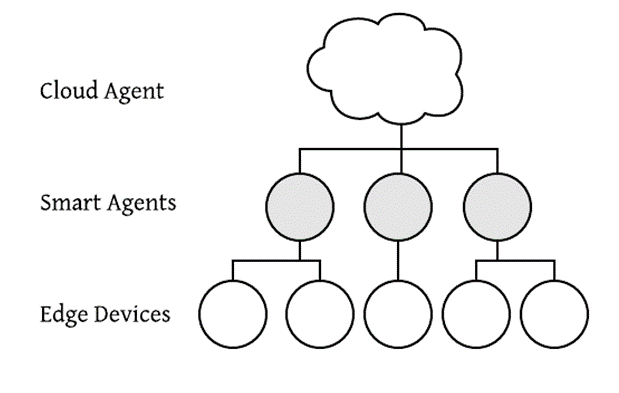
\includegraphics[width=0.7\textwidth]{simplified_architecture}
    \label{fig:simplified_architecture}
    \caption{Architecture diagram}
\end{figure}


\subsection{Communication}

Communication between Smart Agents and Edge Devices is achieved via JSON packets sent over serial while between Smart Agents and the Cloud Agent is via wired and/or wireless TCP/IP network connections.
 
\paragraph{}
We have chosen to use a protocol called MQTT to facilitate communication at this upper layer. MQTT, which stands for Message Queue Telemetry Transport, is a lightweight messaging protocol designed specifically for Internet of Things systems. It relies on a publish-subscribe messaging pattern in which devices may subscribe to a topic to receive any messages subsequently published on it. A MQTT system requires that one device (in this case a machine in the cloud) acts as a broker. The broker is responsible for storing device subscriptions, handling connection status and distributing new messages based on topic.

\subsection{Privacy and security}

mF2C defines three security levels \cite{mf2cwebsite}:

\begin{itemize}
    \item Public: No special protection requirements
    \item Protected: Identity of sender must be proven, but the payload does not need to be encrypted
    \item Private: Identity of sender must be proven, and the payload must be encrypted using strong asymmetric keys.
\end{itemize}

\begin{table}[h!]
    \begin{center}
        \begin{tabular}{ |p{2cm}|p{3cm}|p{3cm}|p{4cm}| } 
            \hline
            Security level & Sender signature & Payload encryption & Example uses \\ \hline
            Public & No & No & Directory of airport shops \\ \hline
            Protected & Yes & No & Flight times \\ \hline
            Private & Yes & Yes & Locations of user's friends \\
            \hline
        \end{tabular}
        \caption{Security levels specification}
        \label{table:secure_levels}
    \end{center}
\end{table}    

Each Agent generates a public/private key pair when it is initialised, or loads one from a file. Rather than have each agent store the public keys of every other device on the network, a Cloud Agent that we call Broker Services facilitates secure message delivery. Each Smart Agent knows only its own public and private keys and the public key of the Cloud Agent. The Cloud Agent maintains a list of all the Smart Agents that have previously connected, their current connection status and their public keys. When Alice wishes to send a message to Bob via her device, her Smart Agent encrypts the message with the Cloud Agent's public key and sends it up the hierarchy. The Cloud Agent then decrypts the message and re-encypts it with Bob's public key before sending it back down the hierarchy to his device.  



\subsection{MQTT Topic Structure}


Using MQTT protocol for secure point-to-point messaging requires careful thinking on the chosen structure of topics. In MQTT, topics are hierarchical and subscription messages allow wildcards, so that if an agent subscribes to \textit{test/\#} (where \# is the wildcard symbol), it receives messages sent to \textit{mf2c}, \textit{mf2c/agent1}, \textit{mf2c/agent2} and \textit{mf2c/agent1/edge1}. Therefore, we assign each agent a number of inboxes. When an agent would like to send a message to another agent, it sends it to that agent's relevant inbox. It also regularly checks its own inboxes for new messages.

\paragraph{}
It also must be possible for one agent to ping any other agent to verify its connection status and speed.

\paragraph{}
For agent1, the inboxes are:
\begin{itemize}
    \item mf2c/agent1/public
    \item mf2c/agent1/public/pingreq
    \item mf2c/agent1/public/pingack
    \item mf2c/agent1/public/handshake
    \item mf2c/agent1/protected
    \item mf2c/agent1/private
\end{itemize}

The Broker Services Cloud Agent has its own public/private key pair and is used to facilitate sending protected and private messages. It has all of the inboxes shown above(with 'broker-services' substituted for 'agent1', but additionally it subscribes to:

\begin{itemize}
    \item mf2c/broker-services/status
    \item mf2c/broker-services/discovery
\end{itemize}


In the topics above, the handshake topic is used for sharing public keys, while the \textit{broker-services/status} message is used by agents reporting a change in their connection status, where connection status is one of:
\begin{itemize}
    \item Connected
    \item Disconnected gracefully (for intentional disconnections; e.g. user logged out)
    \item Disconnected ungracefully (for unintentional disconnections; e.g. loss of internet service)
\end{itemize}

The broker-services/discovery topic is used by the broker to regularly post a list of the agents that have set their visibility appropriately. 

\subsection{Sequence of events}

When a Smart Agent arrives on the network:
\begin{itemize}
    \item The Smart Agent subscribes to its inbox topics
    \item The Smart Agent publishes its new connection status on \textit{mf2c/broker-services/status}
    \item The Smart Agent publishes its public key to \textit{mf2c/broker-services/handshake}
    \item broker-services saves the name of the agent and its public key, then publishes its own key on \textit{mf2c/[agent name]/handshake}
\end{itemize}

While the Smart Agent is on the network:
\begin{itemize}
    \item The Smart Agent checks its inbox topics for new messages
    \item If any of those messages is a ping request (i.e. it was published on topic \textit{mf2c/[agent name]/public/pingreq}), it sends back a ping acknowledgement on \textit{mf2c/[ping source name]/public/pingack}
    \item The Smart Agent returns a list of decrypted message objects to the user
\end{itemize}

When the Smart Agent sends a private message to one or more recipients:
\begin{itemize}
    \item The Smart Agent uses its own private key to sign a hash of its own name and adds this signature to the message
    \item The Smart Agent encrypts the message payload using broker-services' public key
    \item The Smart Agent publishes the packaged message to \textit{mf2c/broker-services/private}
    \item broker-services decrypts the message payload and verifies the signature. It signs the message and encrypts the payload using its own private key.
    \item broker-services publishes the message to each of the recipients private inbox topics (e.g. \textit{mf2c/[destination agent name]/private}
\end{itemize}


When the Smart Agent leaves the network:
\begin{itemize}
    \item It publishes a disconnect message on \textit{mf2c/broker-services/status}
    \item broker-services records that the device has left the network
\end{itemize}
